\documentclass{article}[12pt,a4paper]
\usepackage{a4wide}
\usepackage{tikz}
%\usepackage{fullpage}

\title{Submission Problems}
\author{Richard Douglas}
\date{January 17,  2014}

\begin{document}
  \maketitle
  
  \begin{enumerate}
  \item For the submission problem from the previous week, do the following:
  
  \begin{enumerate}
  \item[(a)]  Use the graphical method to solve the linear program.
  \item[(b)] Suppose that the game designers noticed that players were not casting Fireball
  very often, and have changed the rules in an attempt to balance the game. Now,
  Lightning Bolt and Fireball both score 2000 damage points. Re-solve the problem
  using this new objective function.
  \item[(c)] There are reasons why it may not be appropriate to model this problem as a linear
  program. Identify one of the assumptions that is questionable in this case, and give
  an argument to explain why it is not a reasonable assumption.
  \end{enumerate}
  
  \item A gourmet soup company produces three types of vegetable broth: ready-to-eat, condensed,
  and ultra-condensed. The recipe for the ready-to-eat broth calls for 200 grams of celery, 200
  grams of carrots, and 100 grams of onions for every litre of broth produced, and sells for \$6
  per litre. (You may assume that all other ingredients are in plentiful supply.) The recipe for
  condensed broth calls for 500 grams of celery, 400 grams of carrots, and 300 grams of onions
  per litre, and sells for \$10 per litre. Every litre of ultra-condensed broth requires 800 grams
  of celery, 1 kg of carrots, and 700 grams of onions, and sells for \$34. Before the vegetables
  can be used in the soup, they must be washed and chopped. The preparation cooks are able
  to produce 1.8 kg of celery, 1.6 kg of carrots, and 1 kg of onions per hour. The company
  wants to determine how much of each type of broth it should produce in order to maximize
  its revenue.
  
  \begin{enumerate}
  \item[(a)] Model this problem as an LP in standard form.
  \item[(b)] Convert the constraints into equality constraints, and write out the starting simplex
  tableau for the problem.
  \end{enumerate}
  
  \item 
  
  \begin{enumerate}
  \item[(a)] Let T be a simplex tableau with a feasible basic solution. Prove that if a pivot
  is performed on a row selected using the Minimum Ratio Test, then the resulting
  tableau also has a feasible basic solution.
  \item[(b)] Apply the Simplex Algorithm to the tableau from the January 10 Submission Prob-
  lem. State the optimum solution and its objective value. Describe your results in
  terms of the original problem.
  \end{enumerate}
  
  \end{enumerate}
  \pagebreak
  
  \begin{enumerate}
  
  \item
  \begin{enumerate}
   \item[(a)] 
   \textbf{Sketch}: \newline{}
   
   \begin{center}
   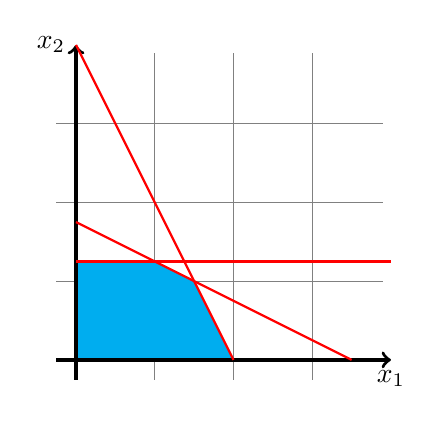
\begin{tikzpicture}[domain=0:4, align=center]
     \draw[very thin, color=gray](-0.25,-0.25) grid(3.9,3.9);
     \filldraw[fill=cyan, draw=red] (0,0) -- (0,1.25) -- (1,1.25) -- (1.5,1) -- (2,0) --  (0,0);
     \draw[very thick, ->] (0,-0.25) -- (0,4) node[left]{$x_2$};
     \draw[very thick, ->] (-0.25,0) -- (4,0) node[below]{$x_1$};
     
     \draw[thick, color=red] (0,1.75) -- (3.5,0);
     \draw[thick, color=red] (0,4) -- (2,0);
     \draw[thick, color=red] (0,1.25) -- (4,1.25);
   \end{tikzpicture}
   \end{center}
   
   \textbf{Corner Points}: 
   $$(0,0), (0,5), (0, 7), (0, 16), (8,0), (14,0), (4,5), (5.5,5), (6,4)$$
   
   \textbf{Feasible Corner Points}:
   $$(0,0), (0,5),  (8,0), (4,5), (6,4)$$
   
   \textbf{Objective Values for $\mathbf{z = 1000x_1 + 3000x_2}$}:
   $$z(0,0) = 0, z(0,5) = 15000, z(8,0) = 8000, z(4,5) = 19000, z(6,4) = 18000$$
   
   \textbf{Conclusion}: The most damage is dealt when Fireball is cast 4 times and Thunderbolt is cast 5 times. \newline{}
   
   \item[(b)] Changing Fireball's damage output to 2000 changes the objective function to
   $$z' = 2000x_1 + 3000x_2$$
   
  The constraints and feasible corner points of the problem remain the same. \newline
  
   \textbf{Objective Values for $\mathbf{z' = 2000x_1 + 3000x_2}$}:
   $$z'(0,0) = 0, z'(0,5) = 15000, z'(8,0) = 16000, z'(4,5) = 23000, z'(6,4) = 24000$$
   
   \textbf{New Conclusion}: Now the most damage is dealt when Fireball is cast 6 times and Thunderbolt is cast 4 times. \newline{}
   
   \item[(c)] While I do find it strange that a dragon would hold still while a wizard is bombarding it with fireballs and lightning bolts,
   while also not fighting back (which could affect the Certainty assumption as a wizard eaten by a dragon in 10 seconds won't really
   have the entire 32 seconds to cast spells for example.) an assumption that I find more questionable is the Divisibility assumption
   as it does not really make sense to partially cast a spell. \newline{}
   
   \textbf{Additional Comments}: Even though modelling this problem using integer programming may make more sense, in both (a) 
   and (b), the optimum values for $x_1$ and $x_2$ were integers. Since the feasible region of the corresponding integer program is 
   a subset of the linear program's feasible region, I think the optimum values of $x_1$ and $x_2$ for the integer program would be 
   identical to those found for the linear program.
   
   Also, we need not be concerned with the Certainty assumption if the wizard is experienced enough so that none of the spells can   
   miss and any damage done by the dragon is negligible. 
  \end{enumerate}
  \pagebreak
  
  \item
  \begin{enumerate}
  \item[(a)] 
  
  \textbf{Decision Variables:} Let $x_1$, $x_2$, $x_3$ represent the number of litres of ready-to-eat, condensed,
  and ultra-condensed broth produced every hour. \newline{}
  
  \textbf{Objective Function:} Ready-to-eat broth sells for \$6 per litre, condensed broth sells for \$10 per litre, and
  ultra-condensed broth sells for \$34 per litre. The company wishes to maximize its revenue. 
  
  The goal is thus to maximize
  
  $$z = 6x_1 + 10x_2 + 34x_3$$
  
  \textbf{Constraints:} Broths require celery, of which up to 1.8 kg or 1800 grams are produced per hour.
  Each litre of ready-to-eat broth requires 200 grams of celery, condensed broth requires 500 grams, and ultra-condensed
  broth requires 800 grams. This gives the constraint
  $$200x_1  + 500x_2 + 800x_3 \le 1800$$
  Similar constraints corresponding to the carrots and onions available are
  $$200x_1 + 400x_2 + 1000x_3 \le 1600$$
  $$100x_1 + 300x_2+ 700x_3 \le 1000$$
  
   The variables must also satisfy the nonnegativity constraints since making a negative amount of broth does not make sense.
   $$x_1 \ge 0, x_2\ge 0, x_3 \ge 0$$ 
   
   \item[(b)] \textbf{Simplified Constraints:} The above inequalities are equivalent to
   $$2x_1  + 5x_2 + 8x_3 \le 18$$
   $$x_1 + 2x_2 + 5x_3 \le 8$$
   $$x_1 + 3x_2+ 7x_3 \le 10$$
   $$x_1 \ge 0, x_2\ge 0, x_3 \ge 0$$ 
   
   \textbf{Equality Constraints:} Introducing slack variables changes the structural constraints to the equalities
    $$2x_1  + 5x_2 + 8x_3 + x_4 = 18$$
   $$x_1 + 2x_2 + 5x_3 + x_5 = 8$$
   $$x_1 + 3x_2+ 7x_3 + x_6 = 10$$
  
  \textbf{Simplex Tableau:}
  \begin{center}
  \begin{tabular}{l | c c c c c c c | c}
             & $z$ & $x_1$ & $x_2$ & $x_3$ & $x_4$ & $x_5$ & $x_6$ & $b$ \\ \hline
  $z$     & $1$ & $-6$   & $-10$ & $-34$  & $0$     & $0$     & $0$     & $0$ \\ \hline
  $x_4$ & $0$ & $2$    & $5$    & $8$      & $1$     & $0$     & $0$     & $18$ \\
  $x_5$ & $0$ & $1$    & $2$    & $5$      & $0$     & $1$     & $0$     & $8$ \\
  $x_6$ & $0$ & $1$    & $3$    & $7$      & $0$     & $0$     & $1$     & $10$ \\
  \end{tabular}
  \end{center}

  \end{enumerate}
  \pagebreak
  \item
  \begin{enumerate}
  \item[(a)]
  \textbf{Proof:} The result holds if after pivoting, all of the variables are nonnegative (because a constraint is violated $\iff$
  at least one variable is negative.) 
  \begin{itemize}
  \item Since all nonbasic variables are set to $0$ in the basic solution, we only need to worry about the
  values of the basic variables after the pivot.
  \item The values of the basic variables are all stored and updated in column $b$.
  \item Let $b_k$ be the entry on the $k$th row of column $b$ \textit{before} the pivot. 
  \item And let $p_k$ be the entry's value \textit{after} the pivot.  
  \item  Let $k$ be $\ge 1$ since the objective value entry of the $b$ column is not of interest.
  \item Let ($i$,$j$) be the choice of pivot row and column. 
  
  \item If $k = i$, then $p_k = b_k/a_{kj} = b_i/a_{ij} \ge 0$ since the pre-pivot basic solution is feasible 
  ($\Rightarrow b_i \ge 0$) and the Minimum Ratio Test requires $a_{ij} > 0$. 
  \item Otherwise $k \ne i$ and $p_k = b_k - a_{kj}b_i/a_{ij} \ge 0$ because $b_i/a_{ij} \le b_k/a_{kj}$
  for $a_{kj} > 0$.
  \item Thus $p_k \ge 0$ for all $k \ge 1$
  \item Therefore after the pivot, the basic variables are all nonnegative and thus the basic solution is feasible. \newline{}
  \end{itemize} 
  
  \item[(b)] 
   \textbf{Starting Tableau:}
   \begin{center}
   \begin{tabular}{l | c c c c c c c | c}
             & $z$ & $x_1$ & $x_2$ & $x_3$ & $x_4$ & $x_5$ & $x_6$ & $b$ \\ \hline
   $z$     & $1$ & $-6$   & $-10$ & $-34$  & $0$     & $0$     & $0$     & $0$ \\ \hline
   $x_4$ & $0$ & $2$    & $5$    & $8$      & $1$     & $0$     & $0$     & $18$ \\
   $x_5$ & $0$ & $1$    & $2$    & $5$      & $0$     & $1$     & $0$     & $8$ \\
   $x_6$ & $0$ & $1$    & $3$    & $7$      & $0$     & $0$     & $1$     & $10$ \\
   \end{tabular}
   \end{center}
   
   \textbf{Pivot at Row 2 Column 1:}
    \begin{center}
    \begin{tabular}{l | c c c c c c c | c}
             & $z$ & $x_1$ & $x_2$ & $x_3$ & $x_4$ & $x_5$ & $x_6$ & $b$ \\ \hline
   $z$     & $1$ & $0$   & $2$ & $-4$  & $0$     & $6$     & $0$     & $48$ \\ \hline
   $x_4$ & $0$ & $0$    & $1$    & $-2$      & $1$     & $-2$     & $0$     & $2$ \\
   $x_1$ & $0$ & $1$    & $2$    & $5$      & $0$     & $1$     & $0$     & $8$ \\
   $x_6$ & $0$ & $0$    & $1$    & $2$      & $0$     & $-1$     & $1$     & $2$ \\
   \end{tabular}
   \end{center}
   
   \textbf{Pivot at Row 3 Column 3:}
    \begin{center}
    \begin{tabular}{l | c c c c c c c | c}
             & $z$ & $x_1$ & $x_2$ & $x_3$ & $x_4$ & $x_5$ & $x_6$ & $b$ \\ \hline
   $z$     & $1$ & $0$   & $4$ & $0$  & $0$     & $4$     & $2$     & $52$ \\ \hline
   $x_4$ & $0$ & $0$    & $2$    & $0$      & $1$     & $-3$     & $1$     & $4$ \\
   $x_1$ & $0$ & $1$    & $-1/2$    & $0$      & $0$     & $7/2$     & $-5/2$     & $3$ \\
   $x_3$ & $0$ & $0$    & $1/2$    & $1$      & $0$     & $-1/2$     & $1/2$     & $1$ \\
   \end{tabular}
   \end{center}
   
   \textbf{Basic Solution:}
   $$x_1 = 3, x_2 = 0, x_3 = 1, x_4 = 4, x_5 = 0, x_6 = 0$$
   
   \textbf{Optimum Value:}
   $$z(3,0,1) = 6*3 + 10*0 + 34*1 = 52$$
   
   \textbf{Conclusion:} To maximize hourly revenue, the gourmet soup company should produce 3 litres of ready-to-eat broth
   and 1 litre of ultra-condensed broth. This will result in an hourly revenue of \$52.
   
  \end{enumerate}
  
  \end{enumerate}
\end{document}